\section{Trabajo a Futuro}
\label{cap:TrabajosFuturos}

Si bien el sistema desarrollado cumple con los objetivos planteados, existen líneas de trabajo que permitirían mejorar sus prestaciones y ampliar su campo de aplicación. En primer lugar, resulta de interés evaluar el sistema en escenarios más complejos y variados, con un número mayor de nodos e incorporando los demás agentes que componen la microrred. Esto permitiría verificar la escalabilidad del esquema distribuido, analizando el impacto sobre las comunicaciones, la latencia en la toma de decisiones y la estabilidad del control a medida que crece el tamaño de la red.

\subsection{Optimización del algoritmo de control de cargas}

Se identifican dos mejoras al algoritmo de gestión implementado. La primera mejora consiste en la \textbf{desconexión anticipada de cargas}. En la versión actual, ante un déficit energético ($I_{total} > I_{disponible}$) es desconedctada una única carga por iteración: la de menor prioridad y, en caso de empate, la de menor consumo. Si esa desconexión no alcanza para restablecer el equilibrio, el sistema debe esperar iteraciones sucesivas, lo que prolonga el estado de sobrecarga. Dado que cada nodo dispone de la información del estado global, se propone que el nodo evalúe dentro de la misma iteración si la desconexión de las cargas de menor jerarquía resulta suficiente y, de no serlo, proceda también a desconectarse sin aguardar una nueva evaluación. De esta forma, la decisión deja de ser estrictamente incremental y pasa a considerar el aporte conjunto de múltiples cargas, reduciendo el tiempo de respuesta y la permanencia en estados transitorios de sobrecarga. La Figura~\ref{img:desconexion_anticipada} compara el comportamiento del algoritmo actual con el de la mejora propuesta. Cabe aclarar que esta mejora no está limitada a cargas de igual prioridad, sino que también puede aplicarse entre niveles distintos, siempre manteniendo el criterio jerárquico establecido.

\begin{figure}[hbt!]
    \centering
    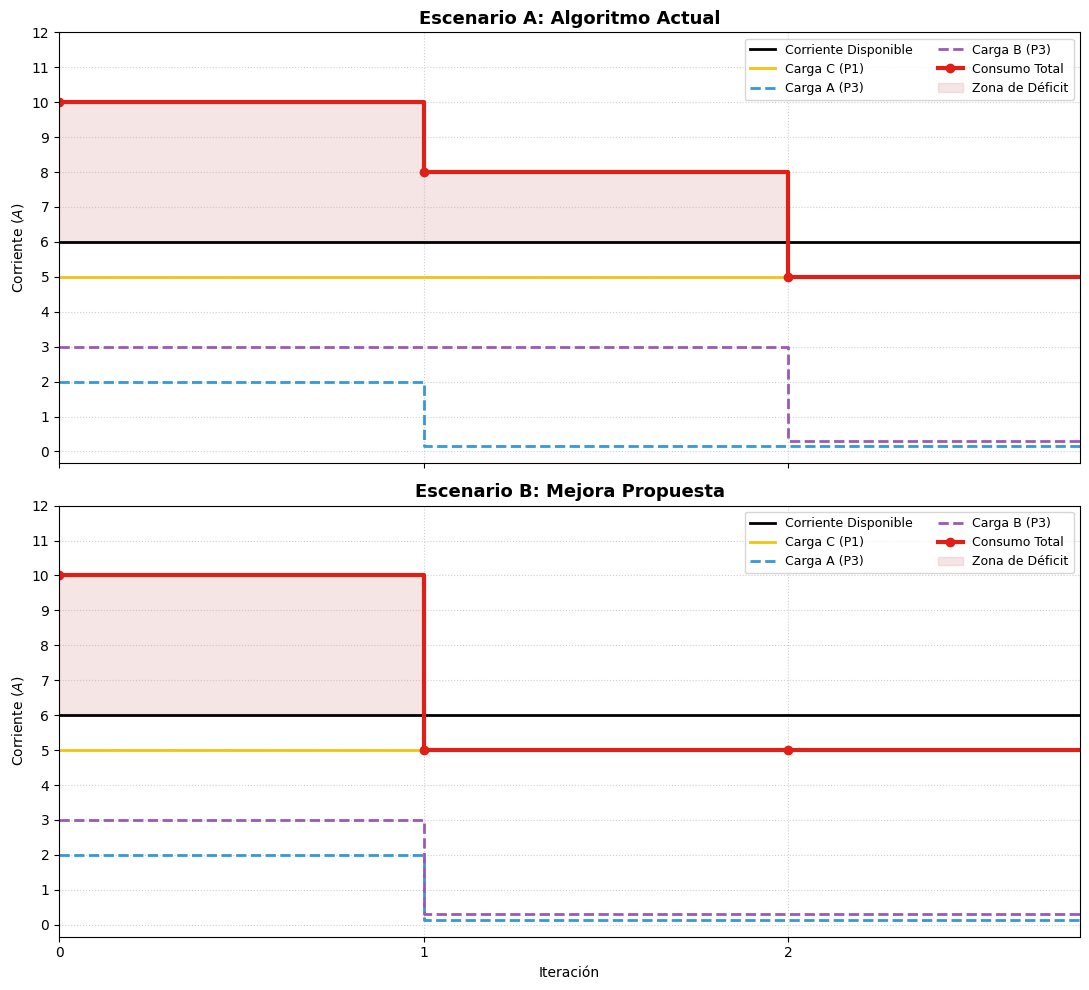
\includegraphics[width=1\textwidth]{imagenes/desconexion-anticipada.png}
    \caption{Comparativa entre algoritmo actual y la mejora propuesta para la desconexión de cargas.}
    \label{img:desconexion_anticipada}
\end{figure}

La segunda mejora considera la \textbf{incorporación de mensajes de solicitud de desconexión}. Con el algoritmo actual pueden producirse configuraciones subóptimas en las que una carga de menor prioridad, por haberse reconectado antes, ocupa la capacidad disponible e impide la reconexión de una carga de mayor prioridad y mayor consumo. Para abordar esta limitación, se propone que un nodo de mayor prioridad, al detectar que podría reconectarse si se liberara capacidad, emita una solicitud de desconexión dirigida a uno o más nodos de menor prioridad. Este mecanismo introduce una forma de negociación entre nodos, en la que las cargas de menor prioridad ceden su lugar en favor de las más relevantes, garantizando la preferencia efectiva de estas últimas en el uso de la energía. La Figura~\ref{img:desconexion_coordinada} ilustra esta situación. Esta función podría implementarse de manera opcional, permitiendo al usuario configurar su activación según las características de las cargas involucradas.

\begin{figure}[hbt!]
    \centering
    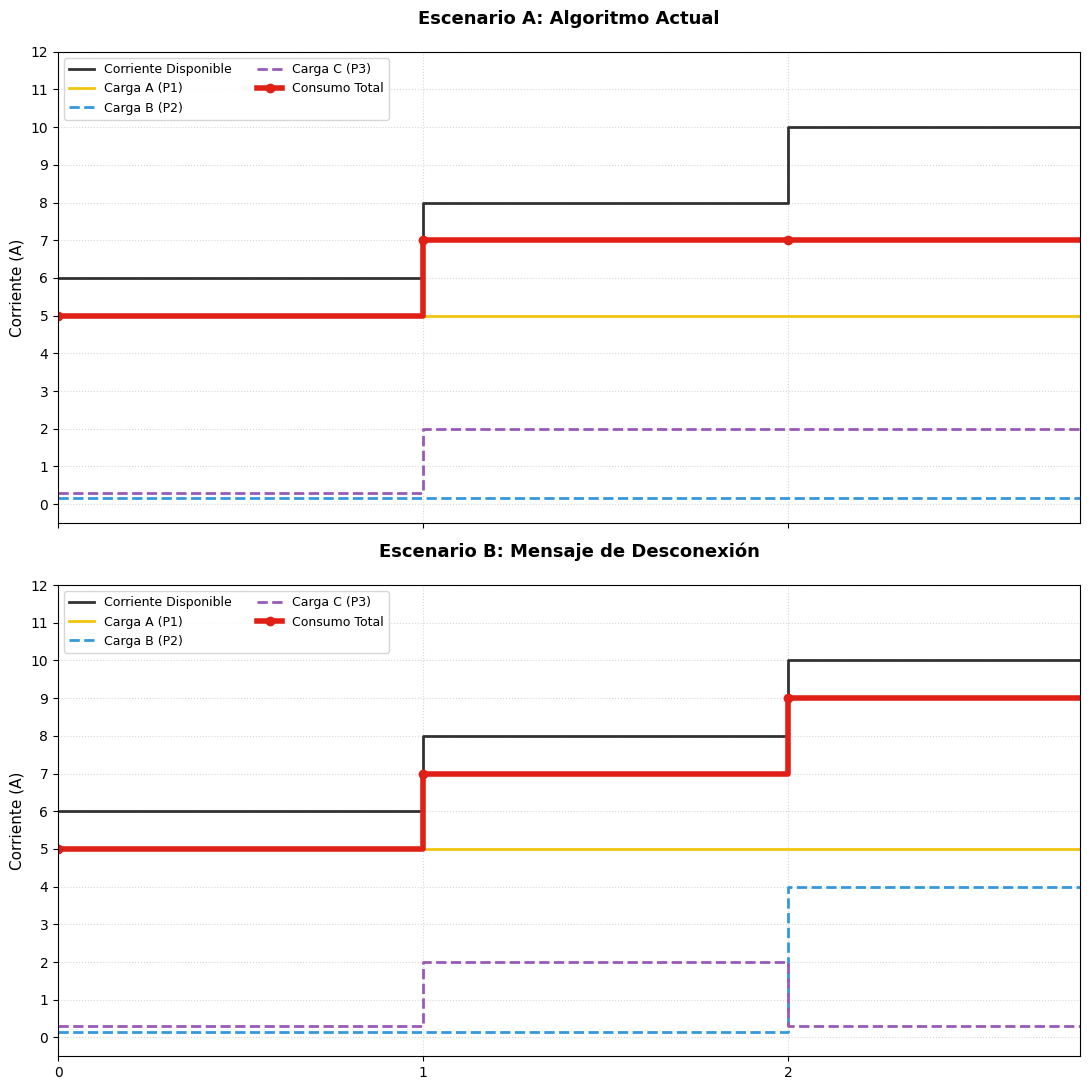
\includegraphics[width=1\textwidth]{imagenes/desconexion-coordinada.png}
    \caption{Comparativa entre algoritmo actual y la implementación de mensajes para la desconexión de cargas.}
    \label{img:desconexion_coordinada}
\end{figure}

\subsection{Mejoras en la Plataforma de Monitoreo}

Se proponen tres funcionalidades que aprovechan la infraestructura de comunicación existente: los cambios de configuración serían publicados desde la plataforma en el \ing{broker} MQTT, el agente de carga se suscribiría a un tópico específico para recibirlos y luego los comunicaría a los nodos de consumo.

\textbf{Cambio remoto de prioridades.} Actualmente la prioridad de cada nodo es configurada de forma física mediante un interruptor tipo DIP, lo que exige una intervención directa sobre el \ing{hardware} y limita la flexibilidad en instalaciones con múltiples nodos. Integrar esta configuración a la plataforma permitiría reasignar prioridades en tiempo real según el contexto operativo, horarios específicos o preferencias del usuario, eliminando la dependencia de configuraciones físicas locales.

\textbf{Modo \textit{deep sleep} programable.} Los nodos permanecen operativos de forma continua, incluso en momentos en los que su participación no es necesaria. Permitir la configuración remota de horarios de bajo consumo, mediante el modo \textit{deep sleep}, reduciría el consumo energético del propio sistema de control. Esta mejora requiere, además de la interfaz de configuración en la plataforma, modificaciones en el \ing{firmware} de los nodos para que gestionen de manera autónoma sus ciclos de activación y suspensión.

\textbf{Análisis del consumo y generación de estadísticas.} La plataforma registra datos históricos, pero no explota completamente su potencial. Mediante el procesamiento de esta información sería posible obtener perfiles de consumo por nodo, patrones horarios e identificación de consumos anómalos, indicadores útiles para mejorar la toma de decisiones del usuario y ajustar prioridades, estrategias de control o políticas de uso. Además, abriría la posibilidad de incorporar a futuro recomendaciones automáticas o estrategias predictivas, alineando la plataforma con las tendencias actuales en gestión energética inteligente.

\subsection{Adaptación del diseño PCB a procesos de manufactura industrial}

Los circuitos impresos del prototipo fueron desarrollados mediante el método de transferencia térmica (planchado), apropiado para etapas iniciales de desarrollo pero limitado en precisión, repetibilidad y calidad eléctrica. Como línea de mejora, se propone el rediseño de las placas para su fabricación profesional, utilizando herramientas de diseño electrónico (EDA) para generar archivos de fabricación estandarizados y contemplando aspectos propios de la manufactura industrial, tales como el dimensionamiento de pistas, la separación entre conductores, la incorporación de serigrafía y el uso de placas multicapa. Esta migración mejoraría la confiabilidad y el desempeño eléctrico del sistema, y habilitaría la producción de múltiples unidades con características homogéneas, facilitando su escalabilidad.

\subsection{Extensión del alcance de comunicación mediante retransmisión entre nodos}
\label{sec:tf_alcance}

Durante los ensayos de alcance descritos en la Sección~\ref{sec:ensayo_alcance}, al probar distancias mayores entre dispositivos pudo observarse el caso típico de nodo oculto: situaciones en las que dos nodos de consumo quedan fuera del alcance radioeléctrico entre sí ---o en las que un nodo deja de recibir directamente al Agente de Carga--- aun cuando ambos mantienen comunicación con un tercer dispositivo intermedio. En la implementación actual, un NC que no recibe la disponibilidad energética publicada por el AC queda excluido de la gestión.

El esquema de consenso implementado en los nodos ofrece una vía natural para superar esta limitación. Dado que cada NC ya difunde periódicamente su estado y participa de la estimación distribuida del consumo total, el mecanismo puede extenderse para que los nodos retransmitan también la disponibilidad energética recibida del AC. De este modo, un NC fuera del alcance directo del AC obtendría dicha información a través de sus vecinos, y la información de un nodo oculto alcanzaría al resto de la red por intermedio de los nodos que sí lo reciben. El alcance efectivo del sistema dejaría así de estar limitado por la cobertura individual de cada enlace, extendiéndose de manera análoga a una red en malla, sin requerir hardware adicional.

La implementación de este mecanismo exige consideraciones adicionales, como el control de duplicados y de lazos de retransmisión (por ejemplo, mediante números de secuencia), el impacto de los saltos múltiples en la latencia de las decisiones y la validación en profundidad del algoritmo de consenso bajo estas topologías, aspectos que quedan planteados como línea de trabajo futuro.